\documentclass[oneside,14pt]{extarticle}
\usepackage[utf8]{inputenc}
\usepackage[english,ukrainian]{babel}
\usepackage{amssymb,amsfonts,amsmath,amsthm,mathtext,textcomp}

\usepackage[includehead, headsep=0pt, footskip=0pt, top=2cm, bottom=2cm, left=2cm, right=1cm]{geometry}
\usepackage{indentfirst}
\usepackage[onehalfspacing]{setspace}
\usepackage[headings]{fancyhdr}
\usepackage{etoolbox}
\usepackage{flafter}
\usepackage{listings}
\usepackage{graphicx}
\usepackage{float}
\usepackage[labelsep=period]{caption}

\usepackage{array}
\fancyhf{}
\renewcommand{\headrulewidth}{0pt}
\pagestyle{fancy}
\fancyfoot[R]{\thepage}
\lstset{breaklines=true,}
\graphicspath{ {./pictures} }

\lstset{
	language=c,
	tabsize=4,
	keepspaces,
	showstringspaces=false,
}
\graphicspath{ {./pictures} }
\setlength{\parindent}{4em}
\setlength\tabcolsep{5px}

\newcommand\subject{Моделювання та аналіз програмного забезпечення}
\newcommand\lecturer{доцент кафедри ПЗ \\ Сердюк П.В.}
\newcommand\teacher{викладач кафедри ПЗ \\ Микуляк А.В.}
\newcommand\mygroup{ПЗ-22}
\newcommand\lab{2}
\newcommand\theme{Класи, інтерфейси і структури у
	мові програмування С\#}
\newcommand\purpose{Ознайомлення з основами класів, структур, та інших базових
	елементів мови програмування С\#}

\begin{document}
\begin{normalsize}
	\begin{titlepage}
		\thispagestyle{empty}
		\begin{center}
			\textbf{МІНІСТЕРСТВО ОСВІТИ І НАУКИ УКРАЇНИ\\
				НАЦІОНАЛЬНИЙ УНІВЕРСИТЕТ "ЛЬВІВСЬКА ПОЛІТЕХНІКА"}
		\end{center}
		\begin{flushright}
			\textbf{ІКНІ}\\
			Кафедра \textbf{ПЗ}
		\end{flushright}
		\vspace{70pt}
		\begin{center}
			\textbf{ЗВІТ}\\
			\vspace{10pt}
			до лабораторної роботи № \lab\\
			\textbf{на тему}: “\textit{\theme}”\\
			\textbf{з дисципліни}: “\subject”
		\end{center}
		\vspace{50pt}
		\begin{flushright}
			
			\textbf{Лектор}:\\
			\lecturer\\
			\vspace{10pt}
			\textbf{Виконав}:\\
			
			студент групи \mygroup\\
			Коваленко Д.М.\\
			\vspace{10pt}
			\textbf{Прийняв}:\\
			
			\teacher\\
			
			\vspace{28pt}
			«\rule{1cm}{0.15mm}» \rule{1.5cm}{0.15mm} 2023 р.\\
			$\sum$ = \rule{1cm}{0.15mm}……………\\
			
		\end{flushright}
		\vspace{\fill}
		\begin{center}
			\textbf{Львів — 2023}
		\end{center}
	\end{titlepage}
		
	\begin{description}
		\item[Тема.] \theme.
		\item[Мета.] \purpose.
	\end{description}

	\section*{Завдання}
	\begin{enumerate}
		\item Реалізувати ланцюжок наслідування у якому б був звичайний клас,
		абстрактний клас та інтерфейс. Перелічіть відмінності та подібності у цих
		структурах у звіті у вигляді таблиці.
		
		\item Реалізувати різні модифікатори доступу. Продемонструвати доступ до цих модифікаторів там де він є, та їх відсутність там, де це заборонено
		(включити в звіт вирізки з скріншотів Intelisense з VisualStudio).
		
		\item Реалізувати поля та класи без модифікаторів доступу. Дослідити який буде доступ	за замовчуванням у класів, структур інтерфейсів, вкладених класів, полів, і т.д. У	звіті має бути відповідна таблиця.
		
		\item Оголосити внутрішній клас з доступом меншим за public. Реалізувати поле цього	типу даних. Дослідити обмеження на модифікатор.
		
		\item Реалізувати перелічуваний тип. Продемонструвати різні булівські операції на перелічуваних типах.
		
		\item Реалізувати множинне наслідування.
		
		\item Реалізувати перевантаження конструкторів базового класу та поточного класу. Показати різні варіанти використання ключових слів base та this. Реалізувати	перевантаження функції.
		
		\item Реалізувати різні види ініціалізації полів як статичних так і динамічних: за	допомогою статичного та динамічного конструктора, та ін. Дослідити у якій послідовності ініціалізуються поля.
		
		\item Реалізувати функції з параметрами out, ref. Показати відмінності при наявності та без цих параметрів. Показати випадки, коли ці параметри не мають значення.
		
		\item Продемонуструвати boxing / unboxing.
		
		\item Реалізувати явні та неявні оператори приведення то іншого типу (implicit та explicit).
		
		\item Реалізувати логіку свого завдання у системі класів.
		
		\item Скопіювати проект і перейменувати всі класи у структури. Дослідити відмінності у класах та структурах та записати їх у вигляді таблиці до звіту. Реалізувати наслідування структур через інтерфейси.
		
		\item Перевизначити і дослідити методи класу object (у тому числі і protected методи).
	\end{enumerate}

	\section*{Хід виконання}
	\subsection*{Частина 1}
	\subsection*{Завдання 1}
	Реалізувати ланцюжок наслідування у якому б був звичайний клас, абстрактний
	клас та інтерфейс. Перелічіть відмінності та подібності у цих структурах у звіті у
	вигляді таблиці
	\begin{figure}[H]
		\centering
		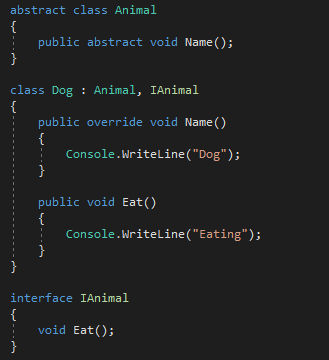
\includegraphics[scale=0.7]{11}
	\end{figure}
		
	\begin{table}[H]
		\centering
		\begin{tabular}{ |c|c|c| }
			\hline
			& \textbf{Class} & \textbf{Abstract Class} \\ 
			\hline
			\textbf{Inheritance} & Single & Single \\ 
			\hline
			\textbf{Fields} & Yes & Yes \\ 
			\hline
			\textbf{Properties} & Yes & Yes \\ 
			\hline
			\textbf{Methods} & Yes & Yes \\ 
			\hline
			\textbf{Constructors} & Yes & Yes \\ 
			\hline
			\textbf{Access Modifiers} & Public, Private, Protected, Internal & Public, Protected, Internal \\ 
			\hline
			\textbf{Instantiation} & Can create objects & Cannot create objects \\ 
			\hline
		\end{tabular}
	\end{table}
	
	\begin{table}[H]
		\centering
		\begin{tabular}{ |c|c| }
			\hline
			& \textbf{Interface} \\ 
			\hline
			\textbf{Inheritance} & Multiple \\ 
			\hline
			\textbf{Fields} & No \\ 
			\hline
			\textbf{Properties} & No \\ 
			\hline
			\textbf{Methods} & Yes \\ 
			\hline
			\textbf{Access Modifiers} & Public \\ 
			\hline
			\textbf{Instantiation} & Cannot create objects \\ 
			\hline
		\end{tabular}
		\caption{Відмінності та подібності класу, абстрактного класу та інтерфейсу.}
	\end{table}
	
	\subsection*{Завдання 2}
	Реалізувати різні модифікатори доступу. Продемонструвати доступ до цих
	модифікаторів там де він є, та їх відсутність там, де це заборонено
	\begin{figure}[H]
		\centering
		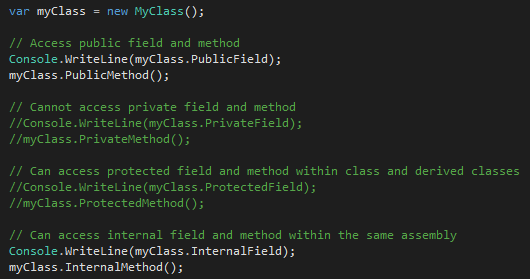
\includegraphics[scale=0.7]{12}
	\end{figure}

	\begin{figure}[H]
		\centering
		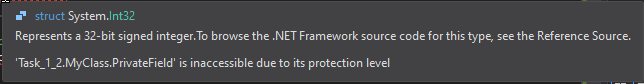
\includegraphics[scale=0.7]{1_2_1}
		\caption{Помилка використання private field.}
	\end{figure}
	
	\begin{figure}[H]
		\centering
		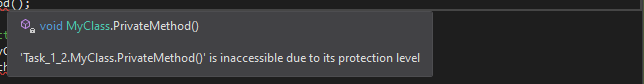
\includegraphics[scale=0.7]{1_2_2}
		\caption{Помилка використання private method.}
	\end{figure}
	
	\begin{figure}[H]
		\centering
		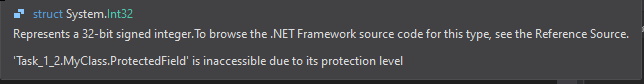
\includegraphics[scale=0.7]{1_2_3}
		\caption{Помилка використання protected field.}
	\end{figure}
	
	\begin{figure}[H]
		\centering
		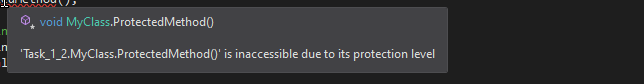
\includegraphics[scale=0.7]{1_2_4}
		\caption{Помилка використання protected method.}
	\end{figure}

	\subsection*{Завдання 3}
	Реалізувати поля та класи без модифікаторів доступу. Дослідити який буде доступ
	за замовчуванням у класів, структур інтерфейсів, вкладених класів, полів, і т.д. У
	звіті має бути відповідна таблиця
	\begin{figure}[H]
		\centering
		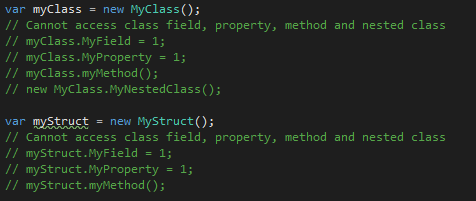
\includegraphics[scale=0.7]{13}
	\end{figure}
	
	Доступом за замовчуванням для всього в C\# є "найбільш обмежений доступ, який ви можете оголосити для цього члена".
	
		\begin{table}[H]
		\centering
		\begin{tabular}{ |c|c| }
			\hline
			\textbf{Member Type} & \textbf{Default Access Modifier} \\ 
			\hline
			namespace & public \\ 
			\hline
			enum & public \\ 
			\hline
			interface & internal \\ 
			\hline
			class & internal \\ 
			\hline
			struct & internal \\ 
			\hline
			delegate & internal \\ 
			\hline
		\end{tabular}
		\caption{Доступ за замовчуванням для не вкладених типів.}
	\end{table}
	
	\begin{table}[H]
		\centering
		\begin{tabular}{ |c|c| }
			\hline
			\textbf{Member Type} & \textbf{Default Access Modifier} \\ 
			\hline
			namespace & public \\
			\hline
			enum & public \\
			\hline
			interface & public \\
			\hline
			class & private \\
			\hline
			struct & private \\
			\hline
			delegate & private \\
			\hline
			constructor & private \\ 
			\hline
			enum member & public\\ 
			\hline
			interface member & public \\ 
			\hline
			method & private \\ 
			\hline
			field & private \\  
			\hline
			property & private \\  
			\hline
		\end{tabular}
		\caption{Доступ за замовчуванням для вкладених типів.}
	\end{table}
		
	\subsection*{Завдання 4}
	Оголосити внутрішній клас з доступом меншим за public. Реалізувати поле цього
	типу даних. Дослідити обмеження на модифікатор
	\begin{figure}[H]
		\centering
		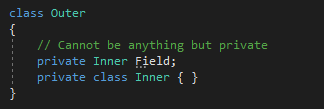
\includegraphics[scale=0.7]{14}
	\end{figure}

	Модифікатор доступу до поля може бути встановленим не більшим ніж модифікатор доступу до типу цього поля.
	
	\subsection*{Завдання 5}
	Реалізувати перелічуваний тип. Продемонструвати різні булівські операції на
	перелічуваних типах
	\begin{figure}[H]
		\centering
		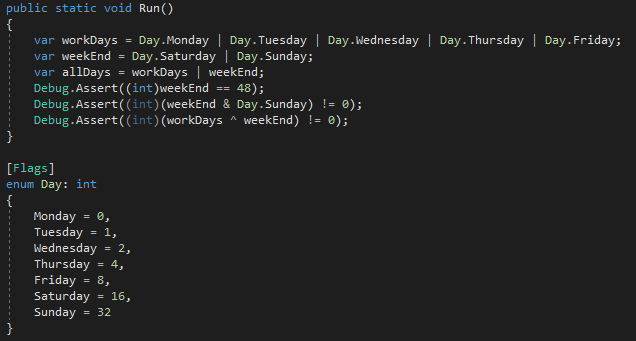
\includegraphics[scale=0.7]{15}
	\end{figure}
	
	\subsection*{Завдання 6}
	Реалізувати множинне наслідування
	\begin{figure}[H]
		\centering
		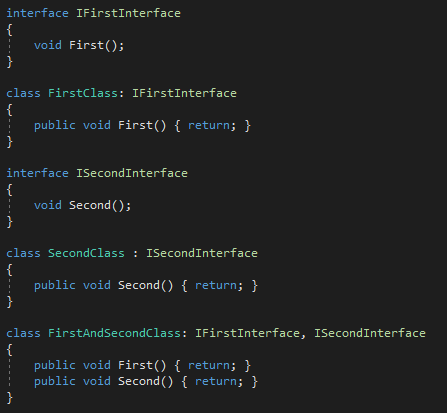
\includegraphics[scale=0.7]{16}
	\end{figure}

	У мові С\# кожен похідний клас може мати лише один базовий клас. Але у багатьох
	випадках це обмеження успішно обходиться за допомогою механізмів інтерфейсів.
	
	\subsection*{Завдання 7}
	Реалізувати перевантаження конструкторів базового класу та поточного класу.
	Показати різні варіанти використання ключових слів base та this. Реалізувати
	перевантаження функції
	\begin{figure}[H]
		\centering
		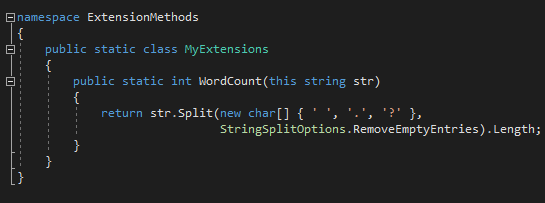
\includegraphics[scale=0.7]{17}
	\end{figure}
	
	Ключове слово $this$ дозволяє перевантажити вказаний конструктор поточного класу. В той час як ключове слово $base$ дозволяє перевантажити вказаний конструктор поточного класу.
	
	\subsection*{Завдання 8}
	Реалізувати різні види ініціалізації полів як статичних так і динамічних: за
	допомогою статичного та динамічного конструктора, та ін. Дослідити у якій
	послідовності ініціалізуються поля
	\begin{figure}[H]
		\centering
		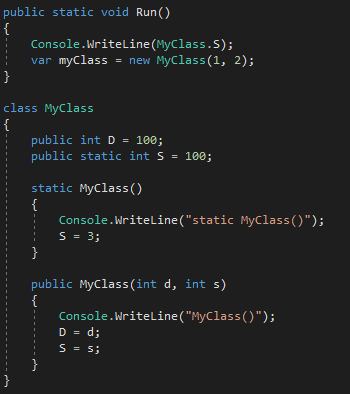
\includegraphics[scale=0.7]{18}
	\end{figure}
	
	\subsection*{Завдання 9}
	Реалізувати функції з параметрами out, ref. Показати відмінності при наявності та
	без цих параметрів. Показати випадки, коли ці параметри не мають значення
	\begin{figure}[H]
		\centering
		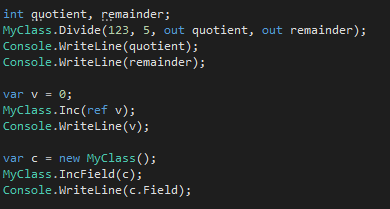
\includegraphics[scale=0.7]{19}
	\end{figure}
	
	\subsection*{Завдання 10}
	Продемонуструвати boxing / unboxing
	\begin{figure}[H]
		\centering
		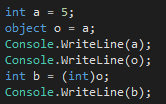
\includegraphics[scale=0.7]{110}
	\end{figure}
	
	\subsection*{Завдання 11}
	Реалізувати явні та неявні оператори приведення то іншого типу (implicit та explicit)
	\begin{figure}[H]
		\centering
		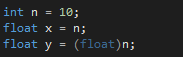
\includegraphics[scale=0.7]{111}
	\end{figure}
	
	\subsection*{Завдання 12}
	Реалізувати логіку свого завдання у системі класів.
	
	\subsection*{Завдання 13}
	Скопіювати проект і перейменувати всі класи у структури. Дослідити відмінності у
	класах та структурах та записати їх у вигляді таблиці до звіту. Реалізувати
	наслідування структур через інтерфейси
	
	\subsection*{Завдання 14}
	Перевизначити і дослідити методи класу object (у тому числі і protected методи)
	\begin{figure}[H]
		\centering
		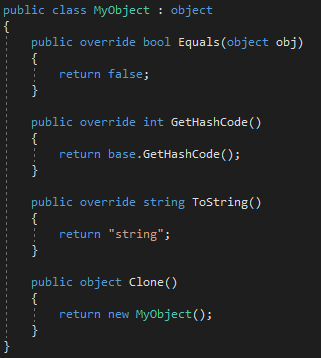
\includegraphics[scale=0.7]{114}
	\end{figure}
	
	\section*{Частина 2}
	\begin{enumerate}
		\item[1)] Дані комп'ютера з параметрами на яких відбулося порівняльне тестування швидкодії та потреб оперативної пам'яті для структур та класів:\\
		Процесор: AMD Ryzen™ 3 PRO 4450U 3.7Ghz, \\ОЗП: 16GiB.
		
		\item[2)] Дані чисельних експериментів
		\begin{table}[H]
			\centering
			\renewcommand*\arraystretch{1.3}
			\begin{tabular}{|p{0.10\linewidth}|p{0.35\linewidth}|p{0.35\linewidth}|}
				\hline
				\textbf{№} & \textbf{Час виклику 10млн віртуальних методів, мс} & \textbf{Час виклику 10млн методів за доп. рефлексії, мс}\\
				\hline
				\textbf{1} & 67 & 10618  \\
				\hline
				\textbf{2} & 140 & 9680  \\
				\hline
				\textbf{3} & 69 & 9748  \\
				\hline
				\textbf{4} & 79 & 9648 \\
				\hline
				\textbf{5} & 178 & 11227 \\
				\hline
				\textbf{Сер.} & 106 & 10184  \\
				\hline
			\end{tabular}
		\end{table}
		
		\item[4)] Висновки. \\
		У C\# виклик методів за допомогою віртуальних методів є значно швидшим, ніж виклик методів за допомогою рефлексії.
		
		Коли ви використовуєте віртуальні методи, компілятор може здійснити прямий виклик до методу, що дозволяє досягти максимальної швидкості виконання. Відповідно, при виклику методів за допомогою рефлексії, потрібно виконати більше додаткової роботи, такої як визначення типів, пошук методів, що призводить до додаткових затрат на час виконання.
	\end{enumerate}
	
	\section*{Результати}
	\begin{table}[h]
		\centering
		\renewcommand*\arraystretch{1.3}
		\begin{tabular}{|p{0.20\linewidth}|p{0.35\linewidth}|p{0.35\linewidth}|}
			\hline
			& \textbf{Класи} & \textbf{Структури}\\
			\hline
			\textbf{Спадковість} & Підтримується спадкування & Можуть реалізовувати тільки інтерфейси \\
			\hline
			\textbf{Алокація пам'яті} & Використовується heap & Використовується stack\\ 
			\hline
			\textbf{Використання} & Використовується для великих об'єктів & Використовується для невеликих об'єктів та структур даних \\ 
			\hline
			\textbf{Передача параметрів} & Передаються по посиланню & Передаються по значенню \\ 
			\hline
			\textbf{Копіювання обєктів} & При передачі та присвоєнні передається посилання & При передачі та присвоєнні передається копіюється об'єкт \\
			\hline
			\textbf{Порівняння об'єктів} & Порівнюються по посиланню & Порівнюються по значенню \\
			\hline
		\end{tabular}
		\caption{Порівняння класів та структур у C\#}
	\end{table}

	\section*{Висновки}
	Під час виконання лабораторної роботи я ознайомився з основами класів, структур, та інших базових елементів мови програмування С\#.
	    
\end{normalsize}
\end{document}
